\documentclass[11pt,a4paper]{article}

\usepackage[utf8]{inputenc}
\usepackage{a4wide}
\usepackage{amsmath,amssymb}
\usepackage{boxproof}
\usepackage{daymonthyear}
\usepackage{float} % for the H placement identifier
\usepackage{multicol}
\usepackage{stmaryrd}
\usepackage{tikz}

%===== SETTINGS =====%

\def\meta#1{\mbox{$\langle\hbox{#1}\rangle$}}
\def\macrowitharg#1#2{{\tt\string#1\bra\meta{#2}\ket}}

{\escapechar-1 \xdef\bra{\string\{}\xdef\ket{\string\}}}

\def\intro#1{{#1}{\cal I}}
\def\elim#1{{#1}{\cal E}}

\showboxbreadth 999
\showboxdepth 999
\tracingoutput 1

\let\imp\to
\def\elim#1{{{#1}{\cal E}}}
\def\intro#1{{{#1}{\cal I}}}
\def\lt{<}
\def\eqdef{\overset{\mathrm{def}}{=\joinrel=}}
\def\eps{\mathrel{\epsilon}}
\def\biimplies{\leftrightarrow}
\def\flt#1{\mathrel{{#1}^\flat}}
\def\setof#1{{\left\{{#1}\right\}}}
\let\implies\to
\def\KK{{\mathsf K}}
\let\squashmuskip\relax

%===== META DATA =====%

\title
{
{\Large Logic in Computer Science}\\
Assignment 6
}
\author
{
	Casper B. Hansen\\
	University of Copenhagen\\
	Department of Computer Science\\
	{\tt fvx507@alumni.ku.dk}
}
\date{\today}

%===== DOCUMENT =====%

\begin{document}

\maketitle

% For testing "old" knowledge:

\section*{2.3.13 \mdseries By natural deduction, show the validity of;}
% 2.3:13 (b)
\subsection*{(b) \mdseries $\forall x{\ }P(a,x,x), \forall x{\ }\forall y{\ }
\forall z{\ }( P(x,y,z) \imp P(f(x),y,f(z)) ) \vdash P(f(a),z,f(f(a)))$}
\begin{proofbox}
	\lbl{1} \:	\forall x{\ }P(a,x,x)					\=\mbox{premise} \\
	\lbl{2} \:	\forall x{\ }
				\forall y{\ }
				\forall z{\ }
				( P(x,y,z) \imp P(f(x),y,f(z)) )		\=\mbox{premise} \\
	\lbl{3} \:	\forall y{\ }
				\forall z{\ }
				( P(a,y,z) \imp P(f(a),y,f(z)) )		\=\elim\forall_x(\ref{2}) \\
	\lbl{4} \:	\forall z{\ }
				( P(a,f(a),z) \imp P(f(a),f(a),f(z)) )	\=\elim\forall_y(\ref{3}) \\
	\lbl{5} \:	P(a,f(a),f(a)) \imp P(f(a),f(a),f(f(a)))\=\elim\forall_z(\ref{4}) \\
	\lbl{6} \:	P(a,f(a),f(a))							\=\elim\forall_x(\ref{1}) \\
	\lbl{7} \:	P(f(a),f(a),f(f(a)))					\=\elim\imp(\ref{5}, \ref{6}) \\
	\lbl{8} \:	\exists P(f(a),z,f(f(a)))				\=\intro\exists(\ref{7}) \\
\end{proofbox}

\section*{3.4.11 \mdseries Find operators to replace the ?, to make the
following equivalences:}
% 3.4:11
\subsection*{(a) \mdseries $\text{AG}(\phi \land \psi) \equiv \text{AG}
\phi{\ }?{\ }\text{AG} \psi$}
The left-hand side of the above states that {\it along all paths all future
states satisfies $\phi \land \psi$}. The logical equivalent can be expressed
as {\it along all paths all future states satisfies $\phi$ and along all paths
all future states satisfies $\psi$}. Hence $\text{AG}(\phi \land \psi) \equiv \text{AG}
\phi{\ }\land{\ }\text{AG} \psi$.

\subsection*{(b) \mdseries $\text{EF} \neg\phi \equiv \neg ?? \phi$}
The left-hand side of the above states that {\it there exists a path from
which, at some point in the future $\phi$ doesn't hold}. The logical
equivalent can be expressed as {\it it is not the case that for all paths,
at some point in the future $\phi$ holds}. Hence $\text{EF} \neg\phi \equiv
\neg \text{AF} \phi$.

\section*{3.7.4 \mdseries Using the function $\text{F}(X)=[\phi] \cup
\text{pre}_\forall(X)$ prove that $[\text{AF}{\ }\phi]$ is the least fixed
point of $F$. Hence argue that the procedure $\texttt{SAT}_{\texttt{AF}}$ is
correct and terminates.}
...

% BDDs:
\section*{6.5.5 \mdseries Given the ordering $[p, q, r]$, compute the reduced
BDDs for $p \land (q \lor r)$ and $(p \land q) \lor (p \land r)$ and explain
why they are identical.}
% 6.5:5
Let us first produce the reduced BBDs for both expressions.
\begin{multicols}{2}
\begin{figure}[H]
        \center
        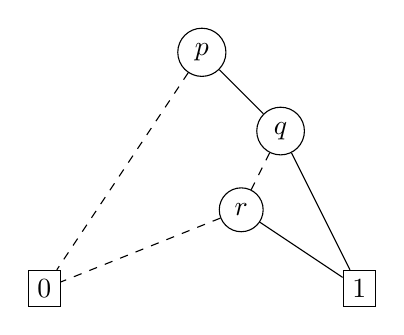
\begin{tikzpicture}
        [
        align=center,
        node/.style={circle, fill=white, draw=black},
        leaf/.style={rectangle, fill=white, draw=black},
        ]
                % nodes
                \node[node] (p) at         (0.0,  0.0) {$p$};
                \node[node] (q) at         (1.0, -1.0) {$q$};
                \node[node] (r) at         (0.5, -2.0) {$r$};
                
                % leaves
                \node[leaf] (0) at         (-2.0, -3.0) {$0$};
                \node[leaf] (1) at         ( 2.0, -3.0) {$1$};
                
                % drawing code
                \foreach \from/\to in {p/q,q/1,r/1} \draw[solid] (\from) -- (\to);
                \foreach \from/\to in {p/0,q/r,r/0} \draw[dashed] (\from) -- (\to);
        \end{tikzpicture}

        \caption{Reduced OBBD for $p \land (q \lor r)$}
\end{figure}
\vfill
\columnbreak
\begin{figure}[H]
        \center
        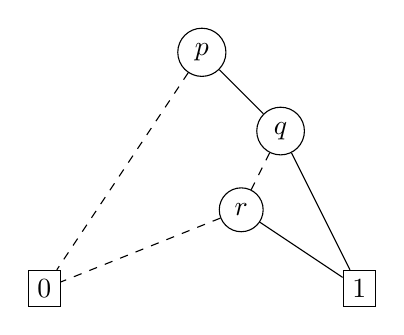
\begin{tikzpicture}
        [
        align=center,
        node/.style={circle, fill=white, draw=black},
        leaf/.style={rectangle, fill=white, draw=black},
        ]
                % nodes
                \node[node] (p) at         (0.0,  0.0) {$p$};
                \node[node] (q) at         (1.0, -1.0) {$q$};
                \node[node] (r) at         (0.5, -2.0) {$r$};
                
                % leaves
                \node[leaf] (0) at         (-2.0, -3.0) {$0$};
                \node[leaf] (1) at         ( 2.0, -3.0) {$1$};
                
                % drawing code
                \foreach \from/\to in {p/q,q/1,r/1} \draw[solid] (\from) -- (\to);
                \foreach \from/\to in {p/0,q/r,r/0} \draw[dashed] (\from) -- (\to);
        \end{tikzpicture}

        \caption{Reduced OBBD for $(p \land q) \lor (p \land r)$}
\end{figure}
\end{multicols}
\noindent We see that they are identical, because in both cases we have that
whenever $\neg p$, we get $0$, hence the first half of the diagram is already
accounted for. And in both cases we need at least one of $q$ and $r$ to
produce a $1$, otherwise $0$. Therefore these two equivalent formulae also
have identical BDDs. 

\section*{6.7.9 \mdseries Let $B_f$ be the OBDD in Figure 6.11 (page 370).
Compute apply $(\oplus,B_f,B_1)$ and reduce the resulting OBDD. If you did
everything correctly, then this OBDD should be isomorphic to the one obtained
from swapping 0- and 1-nodes in Figure 6.11.}
% 6.7:9
...

\newpage
\section*{CTL Model Algorithm \mdseries Supplementary CTL SAT algorithm
exercise}
% Exercise 3.7: 4 (only show the first half,that [[AF \phi]] is the least
% fixpoint of F.)
...

\end{document}